\documentclass[11pt,a4paper]{article}
\usepackage{fontspec}
\setmainfont{DejaVu Sans}[Scale=0.90]
\usepackage{amsmath,amssymb}
\usepackage[margin=2.2cm]{geometry}
\usepackage{booktabs,array,tabularx}
\usepackage{graphicx}
\graphicspath{{../figures/}}
\usepackage{enumitem}
\usepackage{titlesec}
\usepackage{parskip}
\titlelabel{\thetitle.\quad}
\titleformat{\section}{\normalfont\large\bfseries}{\thesection.}{0.6em}{}
\titleformat{\subsection}{\normalfont\normalsize\bfseries}{\thesubsection}{0.6em}{}
\titlespacing*{\section}{0pt}{15pt}{5pt}
\titlespacing*{\subsection}{0pt}{11pt}{4pt}
\setlist[itemize]{leftmargin=1.4em,itemsep=1pt,topsep=3pt}
% Preserve fonts/margins; permit a final line-breaking pass for long prose.
\setlength{\emergencystretch}{2em}
\begin{document}
\begin{center}
{\Large\bfseries Du modèle gris au spectre de l'AlN}\\[4pt]
{\normalsize Moyennes, température et frontières}\\[2pt]
{\small Parties I et III --- 16 septembre 2026}
\end{center}
\section{Résultat et portée}
Les données publiques de Rao et al. (2025) permettent de traiter les douze branches de l'AlN à 300~K : 793 points irréductibles représentent une grille de $24^3$ points. C'est un retraitement de calculs publiés, pas un nouveau calcul ab initio ni une mesure du film du laboratoire.
On établit les sommes spectrales, une trajectoire de capacité harmonique et une comparaison avec une table indépendante de conductivité massive en température. Le dépôt Rao ne sépare pas normal et umklapp : $\tau_N(T)$, $\tau_R(T)$ et la fenêtre hydrodynamique restent à déterminer.
\section{Modes, unités et capacité}
Un mode $\mu=(\mathbf q,s)$ porte $\epsilon_\mu=\hbar\omega_\mu$ et $\mathbf v_\mu=\nabla_{\mathbf q}\omega_\mu$. Les poids irréductibles sont $W_\mu=g_{\mathbf q}/(N_qV_0)$, avec $\sum g_{\mathbf q}=N_q$.
\[x_\mu=\hbar\omega_\mu/(k_BT),\qquad C_\mu=W_\mu k_B\frac{x_\mu^2e^{-x_\mu}}{(1-e^{-x_\mu})^2},\qquad C=\sum_\mu C_\mu.\]
La limite par oscillateur à $x=0$ est $k_B$. Les trois translations à $\Gamma$ sont incluses dans $C$, avec zéro transport sur cette grille. Leur poids dans $C(300\,{\rm K})$ vaut $3{,}01\,10^{-5}$.
Les vecteurs réciproques donnent $V_0=(2\pi)^3/|\det(\mathbf b_1,\mathbf b_2,\mathbf b_3)|=4{,}09299\,10^{-29}$ m$^3$. Conversions vérifiées : rad/ps vers rad/s, km/s vers m/s, ps$^{-1}$ vers s$^{-1}$. Les figures utilisent $\omega/(2\pi)$ en THz, distinct de la fréquence FDTR.
Pour le cristal uniaxe avec $z$ parallèle à $c$, on somme $v_c^2=v_z^2$ et $v_a^2=(v_x^2+v_y^2)/2$. Ces quantités respectent les symétries de la grille irréductible ; les seuls $v_x^2$ des représentants ne suffisent pas en général.
Les colonnes sont des indices de branche. Les trois premières sont acoustiques près de $\Gamma$. Une attribution LA/TA/LO/TO sur tout le spectre demanderait les vecteurs propres, notamment aux croisements.
\section{Deux moyennes pour deux observables}
Dans l'approximation diagonale des temps de relaxation (RTA),
\[\delta n_\mu=-\tau_\mu\mathbf v_\mu\cdot\nabla T\,\partial_Tn_\mu^0,\qquad \kappa_{ij}=\sum_\mu C_\mu v_{\mu i}v_{\mu j}\tau_\mu.\]
Les taux disponibles vérifient $r=r_{\rm anh}+r_{\rm iso}$, $\tau=1/r$. La partie anharmonique comprend normal et umklapp : $\tau$ n'est ni $\tau_N$ ni $\tau_R$. Les fichiers \texttt{plus/minus} séparent absorption et émission, pas normal et umklapp.
Posons $A_\mu=C_\mu v_{\mu i}^2$. Une durée reproduit la conductivité statique, une autre la pente de sa réponse RTA de Laplace :
\[\tau_{{\rm stat},i}=\frac{\sum A_\mu\tau_\mu}{\sum A_\mu},\qquad \kappa_i(p)=\sum_\mu\frac{A_\mu\tau_\mu}{1+p\tau_\mu}=\kappa_i(0)[1-p\tau_{{\rm mem},i}+O(p^2)],\]
\[\tau_{{\rm mem},i}=\frac{\sum A_\mu\tau_\mu^2}{\sum A_\mu\tau_\mu}\ \ge\ \tau_{{\rm stat},i}.\]
La dernière inégalité découle de Cauchy--Schwarz ; l'égalité exige une durée commune aux modes de poids non nul. La mémoire ajuste une pente, pas toute la réponse. Le développement affiché est valable sur la grille finie ; dans le continuum, sa pente et son reste demandent la convergence des moments inverses correspondants (note 18). Aucun des deux temps n'est automatiquement un temps GK.
\begin{center}\begin{tabular}{@{}lrr@{}}\toprule
Rao, 300 K & Plan basal & Axe $c$\\\midrule
$\kappa^{\rm RTA}$ (W\,m$^{-1}$K$^{-1}$) & 309,775 & 302,443\\
$\kappa^{\rm itérative}$ fournie & 344,25 & 342,68\\
$\tau_{\rm stat}$ (ps) & 24,01 & 20,58\\
$\tau_{\rm mem}$ (ps) & 149,30 & 231,66\\\bottomrule
\end{tabular}\end{center}
On retrouve $C=2{,}434256\,10^6$ J\,m$^{-3}$K$^{-1}$. L'écart aux sorties du dépôt est inférieur à $0{,}003\,\%$ pour $\kappa$ et $0{,}0001\,\%$ pour $C$. Cela vérifie le traitement, pas la convergence du calcul physique. Les moments en $\tau^2$ sont sensibles aux modes longs.
\section{Fermeture spectrale conservatrice}
Avec des taux variables, deux cibles utilisant la même température énergétique ne garantissent pas la conservation. Introduisons
\[y_\mu=\frac{\sqrt{W_\mu}\delta n_\mu}{\sqrt{n_\mu^0(1+n_\mu^0)}},\quad e_\mu=\epsilon_\mu\sqrt{W_\mu n_\mu^0(1+n_\mu^0)},\quad P_{\mu j}=\hbar q_{\mu j}\sqrt{W_\mu n_\mu^0(1+n_\mu^0)}.\]
Ces opérateurs se construisent sur la zone complète, avec les vecteurs dans une première zone de Brillouin cohérente, ou après reconstruction explicite des symétries. Les seuls représentants irréductibles ne suffisent pas pour les moments de quasi-moment. Les translations demandent un traitement par limite. Pour $D_N=\mathrm{diag}(r_{N,\mu})$ et $H_N=(e,P_x,P_y,P_z)$, une relaxation projetée conservatrice s'écrit
\[{\cal C}_N=D_N-D_NH_N(H_N^TD_NH_N)^+H_N^TD_N.\]
Pour ${\cal C}_R$, conserver seulement $H_R=e$. On a $H_N^T{\cal C}_Ny=0$ et $e^T{\cal C}_Ry=0$. Avec $U=D^{1/2}H$, l'opérateur devient $D^{1/2}[I-U(U^TU)^+U^T]D^{1/2}$ : symétrique positif semi-défini. Le code applique cette projection sans matrice dense. C'est un modèle de relaxation, pas la matrice ab initio des collisions : les diagonales ne fixent pas les couplages. La projection modifie aussi la diagonale de départ ; ses taux sont des paramètres avant projection, pas la diagonale finale. L'identité de pseudo-inverse et les limites de cette interprétation sont auditées dans la note 18.
Pour un opérateur complet ${\cal C}$ et $b_{\mu i}=\epsilon_\mu v_{\mu i}\sqrt{W_\mu n_\mu^0(1+n_\mu^0)}$, sur le sous-espace dissipatif,
\[\kappa_i(p)=\frac{b_i^T({\cal C}+pI)^{-1}b_i}{k_BT^2},\qquad \tau_{{\rm mem},i}=\frac{b_i^T{\cal C}^{-2}b_i}{b_i^T{\cal C}^{-1}b_i}.\]
Un invariant restant couplé au flux peut empêcher une conductivité DC finie. Dans une limite de dérive lente $y\simeq P\mathbf a$, les matrices $S=P^TP$ et $M=P^T{\cal C}_RP$ donnent $S\dot{\mathbf a}=-M\mathbf a$ en géométrie uniforme. Les taux sont les valeurs propres généralisées de $(M,S)$.
La viscosité demande encore l'élimination des modes rapides couplés par le transport spatial et une séparation d'échelles vérifiée. Le flux n'est plus proportionnel au quasi-moment par une vitesse unique : remplacer deux temps par des moyennes dans $\tau_\ell=4\tau_N/5$ ne constitue pas une fermeture spectrale.
\section{Température}
La table ShengBTE de \emph{Phonon Olympics} fournit une trajectoire massive indépendante, RTA et itérative. Le fichier de contrôle associé désactive les isotopes. Les taux Rao ne sont pas renormalisés sur elle. La figure retient 100--1000~K ; 20~K est indisponible. Les valeurs 30--75~K sont archivées sans certification de convergence ici.
\begin{center}\begin{tabular}{@{}rrrrr@{}}\toprule
$T$ (K) & RTA basal & RTA $c$ & Itératif basal & Itératif $c$\\\midrule
100 & 2690,63 & 2459,81 & 3481,10 & 3329,53\\
300 & 270,90 & 251,05 & 298,37 & 290,97\\
600 & 108,57 & 101,16 & 119,55 & 116,94\\
1000 & 62,07 & 57,95 & 68,33 & 66,89\\\bottomrule
\end{tabular}\end{center}
Unités : W\,m$^{-1}$K$^{-1}$. Une régression des points RTA suivant $c$ entre 400 et 1000~K donne $\kappa_c\propto T^{-1{,}144}$. Ce sont des calculs massifs, pas une loi de film.
Indépendamment, $C(T)$ est recalculée à fréquences Rao fixes : approximation harmonique sans dilatation. Les durées à 300~K ne sont pas réutilisées pour inventer $\kappa(T)$. À 300~K, les indices 4--12 représentent 63,77~\% de $C$ et 18,80~\% de $\kappa_c^{\rm RTA}$.
\begin{center}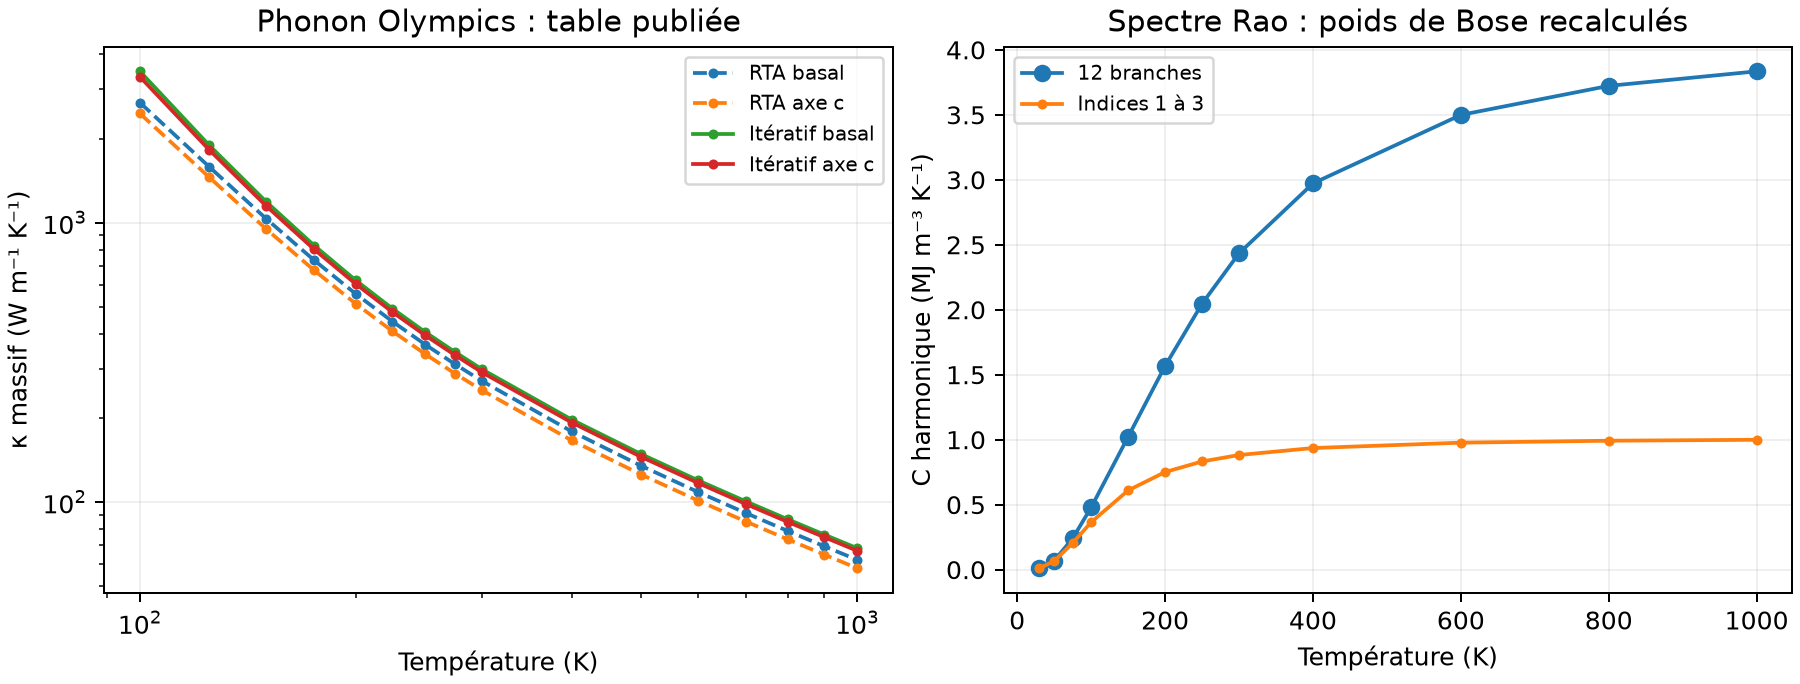
\includegraphics[width=\textwidth]{08_aln_temperature.png}\end{center}
Les lois de Morelli--Callaway restent une option approchée. Le tableau global de Morelli--Slack ne fournit pas les taux $N/U$ par branche nécessaires. Ajuster $\kappa(T)$ seule ne les identifie pas. Les asymptotiques de Ma et al. ne coïncident pas toutes avec un Debye--Callaway usuel : aucun raccord arbitraire n'est effectué.
\section{Épaisseur et surfaces}
Avec les durées RTA disponibles,
\[\Lambda_{\mu z}=|v_{\mu z}|\tau_\mu,\quad K_{\mu z}=\Lambda_{\mu z}/d,\qquad F_i(K>k)=\frac{\sum_{K_{\mu z}>k}C_\mu v_{\mu i}^2\tau_\mu}{\kappa_i}.\]
Ces fractions portent sur le transport massif RTA, pas sur un nombre de phonons ou une conductivité de film.
\begin{center}\begin{tabular}{@{}lrr@{}}\toprule
Épaisseur & $F_c(K>0{,}1)$ & $F_c(K>1)$\\\midrule
500 nm & 78,65 \% & 34,82 \%\\
5 $\mu$m & 34,82 \% & 7,30 \%\\
20 $\mu$m & 16,46 \% & 0 \% sur cette grille\\\bottomrule
\end{tabular}\end{center}
Le zéro n'exclut pas des modes plus longs dans le continuum. Les quantiles 10, 50, 90~\% du poids $\kappa_c$ sont 29,0~nm, 161,3~nm et 3,43~$\mu$m, non représentés par une unique longueur grise.
\subsection{Un problème de frontières calculable}
Pour un gradient constant parallèle au film, des parois identiques réfléchissantes de spécularité $p_s$ et la RTA stationnaire,
\[S(K,p_s)=1-\frac{(1-p_s)K(1-e^{-1/K})}{1-p_s e^{-1/K}},\qquad \kappa_\parallel=\sum_\mu C_\mu v_{\mu a}^2\tau_\mu S(K_{\mu z},p_s).\]
Le déficit au flux massif décroît comme $e^{-z/(|v_z|\tau)}$. Les réflexions donnent une série géométrique de raison $p_s e^{-1/K}$ ; la moyenne sur $z$ donne le numérateur. Les limites sont $S(0,p_s)=1$ et $S(K,1)=1$. La moyenne angulaire isotrope retrouve Fuchs--Sondheimer.
À 500~nm, on obtient 231,64, 258,57 et 309,78 W\,m$^{-1}$K$^{-1}$ pour $p_s=0$, $0{,}5$ et $1$. Scénarios de conduction \emph{parallèle}, ils ne prédisent pas directement FDTR transversal, la transmission vers un substrat ou un écoulement collectif. La spécularité n'est pas mesurée. Aucun taux de frontière n'est ajouté avant cette suppression : on compterait deux fois les mêmes surfaces.
\begin{center}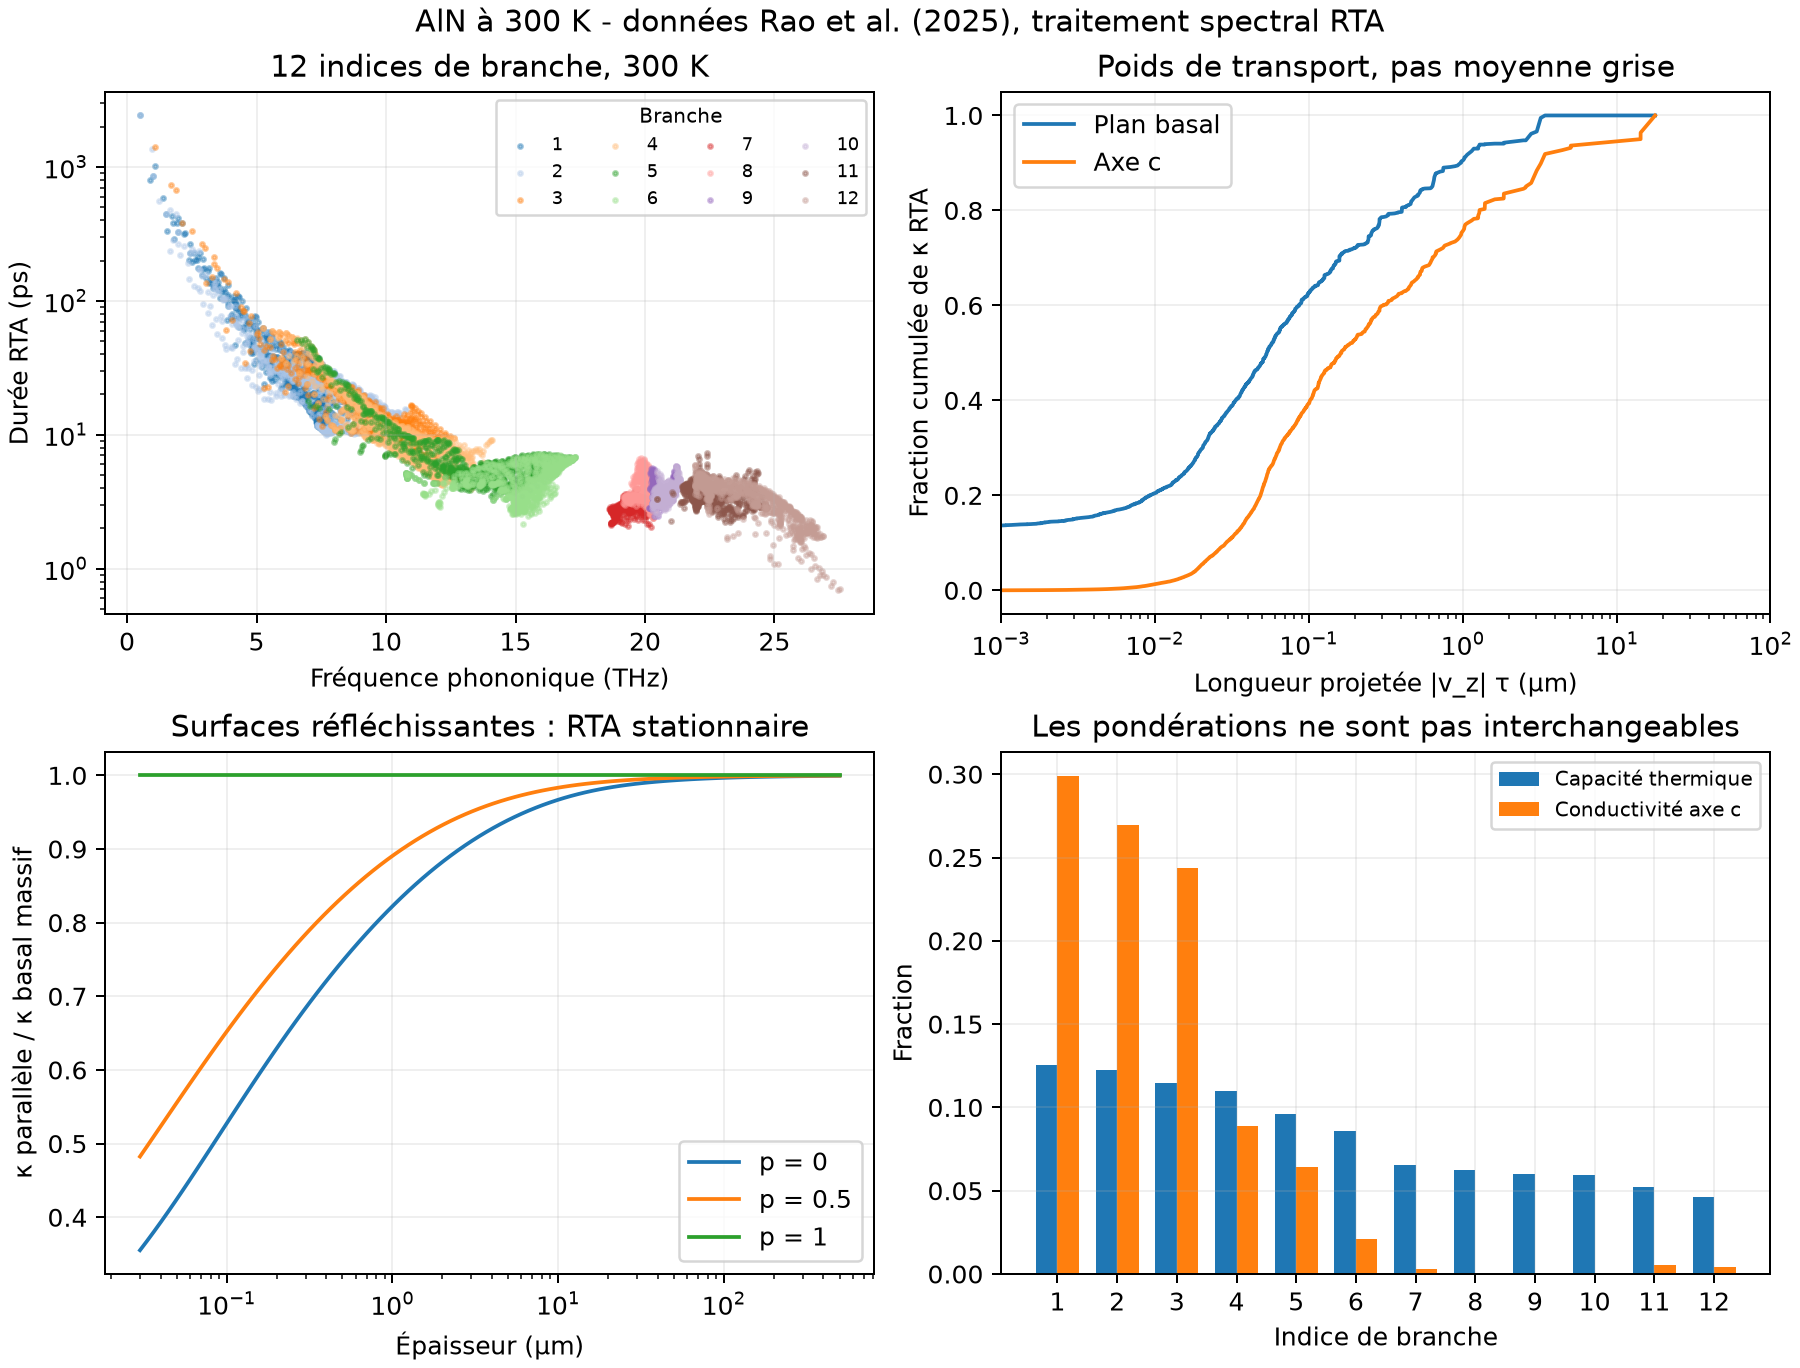
\includegraphics[width=0.95\textwidth]{07_aln_spectral.png}\end{center}
\subsection{Convergence}
Le premier mode positif est à 0,499~THz ; les fréquences inférieures ne sont pas résolues. Environ 12,97~\% du poids basal a $v_z$ nul à la précision numérique. Le poids fini de ces modes rasants sur une grille peut fausser la limite des films très minces. Les accumulations, moments temporels, basses températures et faibles épaisseurs demandent une convergence propre. Reproduire $\kappa$ ne suffit pas.
Pour FDTR, profondeur de pénétration, faisceaux et gradients interfaciaux sont aussi des échelles pertinentes ; $\Lambda/d$ seul ne contrôle pas l'erreur d'un modèle local.
\section{Temps de vol et temps visqueux}
Des taux séparés permettraient de comparer les processus du même mode, avec pondération explicitée. Le code rapporte une fraction satisfaisant un ordre fort (facteur 10 par défaut), pas une preuve d'hydrodynamique : il faut vérifier le sous-espace lent de l'opérateur.
Le temps $d/|v_z|$ est un temps de vol. Dans un canal collectif, le quasi-moment atteint la paroi par diffusion visqueuse :
\[\nu_{\rm ph}\sim v^2\tau_N,\qquad t_{\rm paroi}^{\rm visc}\sim d^2/\nu_{\rm ph}.\]
Une fenêtre de Poiseuille à parois diffusantes demande schématiquement $\tau_N\ll t_{\rm paroi}^{\rm visc}\ll\tau_R$, soit
\[v\tau_N\ll d\ll v\sqrt{\tau_N\tau_R},\]
à facteurs géométriques près. L'ordre de vol libre $v\tau_N\ll d\ll v\tau_R$ de la carte précédente est plus faible. Ce critère de canal ne se transpose pas sans résolution au film chauffé transversalement.
\section{Reproduction et suite}
Les données converties, empreintes SHA-256, attribution et résultats sont dans \texttt{theory/aln/}. Les scripts \texttt{prepare\_aln\_sources.py} et \texttt{analyse\_aln\_spectrum.py} séparent acquisition et analyse ; analyse et tests fonctionnent hors ligne. Les tests couvrent la dérivée de l'énergie, Debye en $T^3$, la mémoire, les invariants et la positivité des collisions, une intégration indépendante du transport entre parois et les sorties publiées $C,\kappa$.
Pour terminer quantitativement : taux $N/U$ séparés en température, composition et défauts spécifiés, convergence des moments, opérateur de collision ou projection validée, puis conditions interfaciales réelles. Phonon Olympics fournit des constantes de force pour un nouveau calcul BTE ; ce calcul et sa séparation $N/U$ n'ont pas été exécutés ici.
\section{Sources}
\begin{enumerate}
\item X. Rao et al., Mendeley Data V1 (2025), doi:\allowbreak 10.17632/\allowbreak w9hg2mnnwy.1, CC BY 4.0. Sous-ensemble AlN converti ; archive contrôlée.
\item A. J. H. McGaughey et al., \emph{Phonon Olympics}, J. Appl. Phys. \textbf{138}, 135108 (2025), doi:\allowbreak 10.1063/\allowbreak 5.0289819. Table auteur, version fixée dans le manifeste.
\item J. Ma, W. Li et X. Luo, Phys. Rev. B \textbf{90}, 035203 (2014), doi:\allowbreak 10.1103/\allowbreak PhysRevB.90.035203.
\item D. T. Morelli et G. A. Slack, \emph{High Lattice Thermal Conductivity Solids}, chapitre consulté via le dépôt pédagogique de Cornell.
\item N. K. Ravichandran et A. J. Minnich, Phys. Rev. B \textbf{93}, 035314 (2016), doi:\allowbreak 10.1103/\allowbreak PhysRevB.93.035314. Transport dans les films et suppression stationnaire.
\item W. Li et al., ShengBTE, Comput. Phys. Commun. \textbf{185}, 1747--1758 (2014). Formats confrontés à la documentation, puis contrôlés par reconstruction des sorties du dépôt.
\end{enumerate}
\end{document}